\section{Models}

We implemented the RSP formulation ideas above on a simple aircraft design problem that is systematically developed in~\cite{Ozturk2018}.
We optimize a wing, fuselage, and engine given a payload and range requirement. A short qualitative overview of the model follows; for
more detailed information, please refer to~\cite{Ozturk2018}.

\subsection{Flight Profile}

The flight profile models have been borrowed from ~\cite{York2018}. Within the model, the
trajectory of the aircraft is optimized over five flight segments,
although we are restricted to modeling only climb segments
and therefore the stored gravitational potential energy of the aircraft is not captured.

\subsection{Atmosphere}

The atmosphere model is taken from~\cite{Tao2018}, and considers changes in density and dynamic
viscosity with altitude, for a standard atmosphere.

\subsection{Aircraft}

The aircraft is simply modeled as a wing, fuselage and engine. The aircraft is assumed
to be in steady flight, so that the thrust power is equal to the sum of the drag power and rate of change
of potential energy of the aircraft, and the lift is equal to the total weight, ignoring the vertical component of
thrust in climb. Its total weight is the sum of its components, as shown in Figure~\ref{fig:liftweight}.
The aircraft has to be able to takeoff at specified minimum speed without stallingas well.
Its component models are detailed below.

\subsubsection{Wing}

Lift is generated by the wing, as a function of its geometry and freestream conditions.
The wing structure model is based on a simple beam model with a distributed lift load,
and a point mass in the center representing the fuselage, as shown in Figure~\ref{fig:liftweight}.
Wing fuel volume is modeled as a fraction of the total internal volume. Its drag is
approximated simply as a sum of the induced and profile drags, the latter of which is estimated using a
form factor which is uncertain. The weight of the wing is the sum of skin and spar weights.

\subsubsection{Fuselage}

The fuselage is assumed to only contain fuel, but is lower bounded from below at a small value.
The fuselage drag is exactly proportional to its frontal area.
The fuselage is assumed not to contain any structural members, and so its weight consists only of skin weight.

\subsubsection{Engine}

The aircraft is powered by a naturally aspirated piston engine. It is subject to
power lapse at lower air densities at higher altitudes. Its weight is modeled using a posynomial fit of existing
engines. Its \gls{bsfc} is modeled as a function of maximum thrust at a given altitude.


\begin{figure}
\centering
\caption{\label{fig:liftweight} Wing lift is equal and opposite to the wing weight, payload weight, and total fuel weight.}
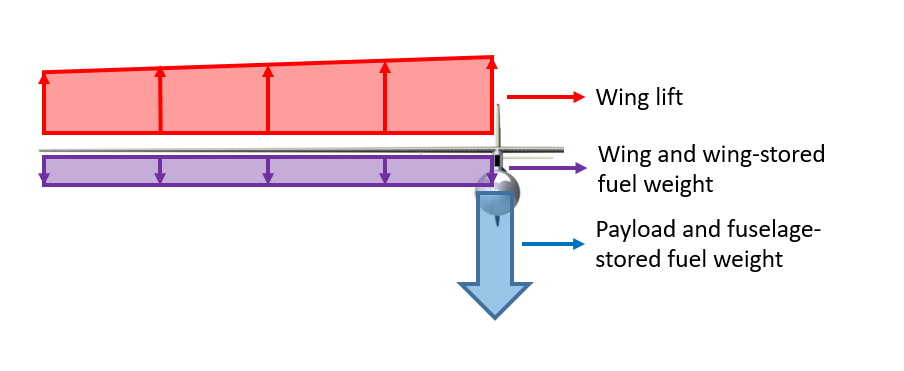
\includegraphics[width=0.8\textwidth]{liftweight.PNG}
\end{figure}

\subsection{Source of non-log-convexity: fuel volume}
We have already detailed the fuel models in the wing and fuselage sections, but it is noteworthy that
the signomial constraint in the optimization appears in the aircraft total fuel volume constraint,
as shown in Equation~\ref{eq:fuel}:

\begin{equation}
\label{eq:fuel}
V_f \leq V_{f_{wing}} + V_{f_{fuse}} 
\end{equation}
